\chapter{Literature review}
\label{literature_review}


\citep{Abegaz_2024} esxample.

This review assesses where the science currently stands to enable the development of a prototype forecasting system that provides medium-range predictions of areas at risk of flash flooding over a continuous global domain. As outlined in Figure \ref{fig:literature_structure}, each thematic section in this chapter is examined through three analytical lenses: \textit{Progress} charts the evolution of knowledge, \textit{Barriers} articulates the limitations that persist or remaining research gaps, and \textit{Opportunities} distils these gaps into the research questions that guide this thesis. By moving systematically from established achievements through current challenges and to future prospects, the chapter positions the reader to understand both the state of the art and the rationale for the analyses presented in the subsequent chapters.

\begin{figure}[htbp]
\centering
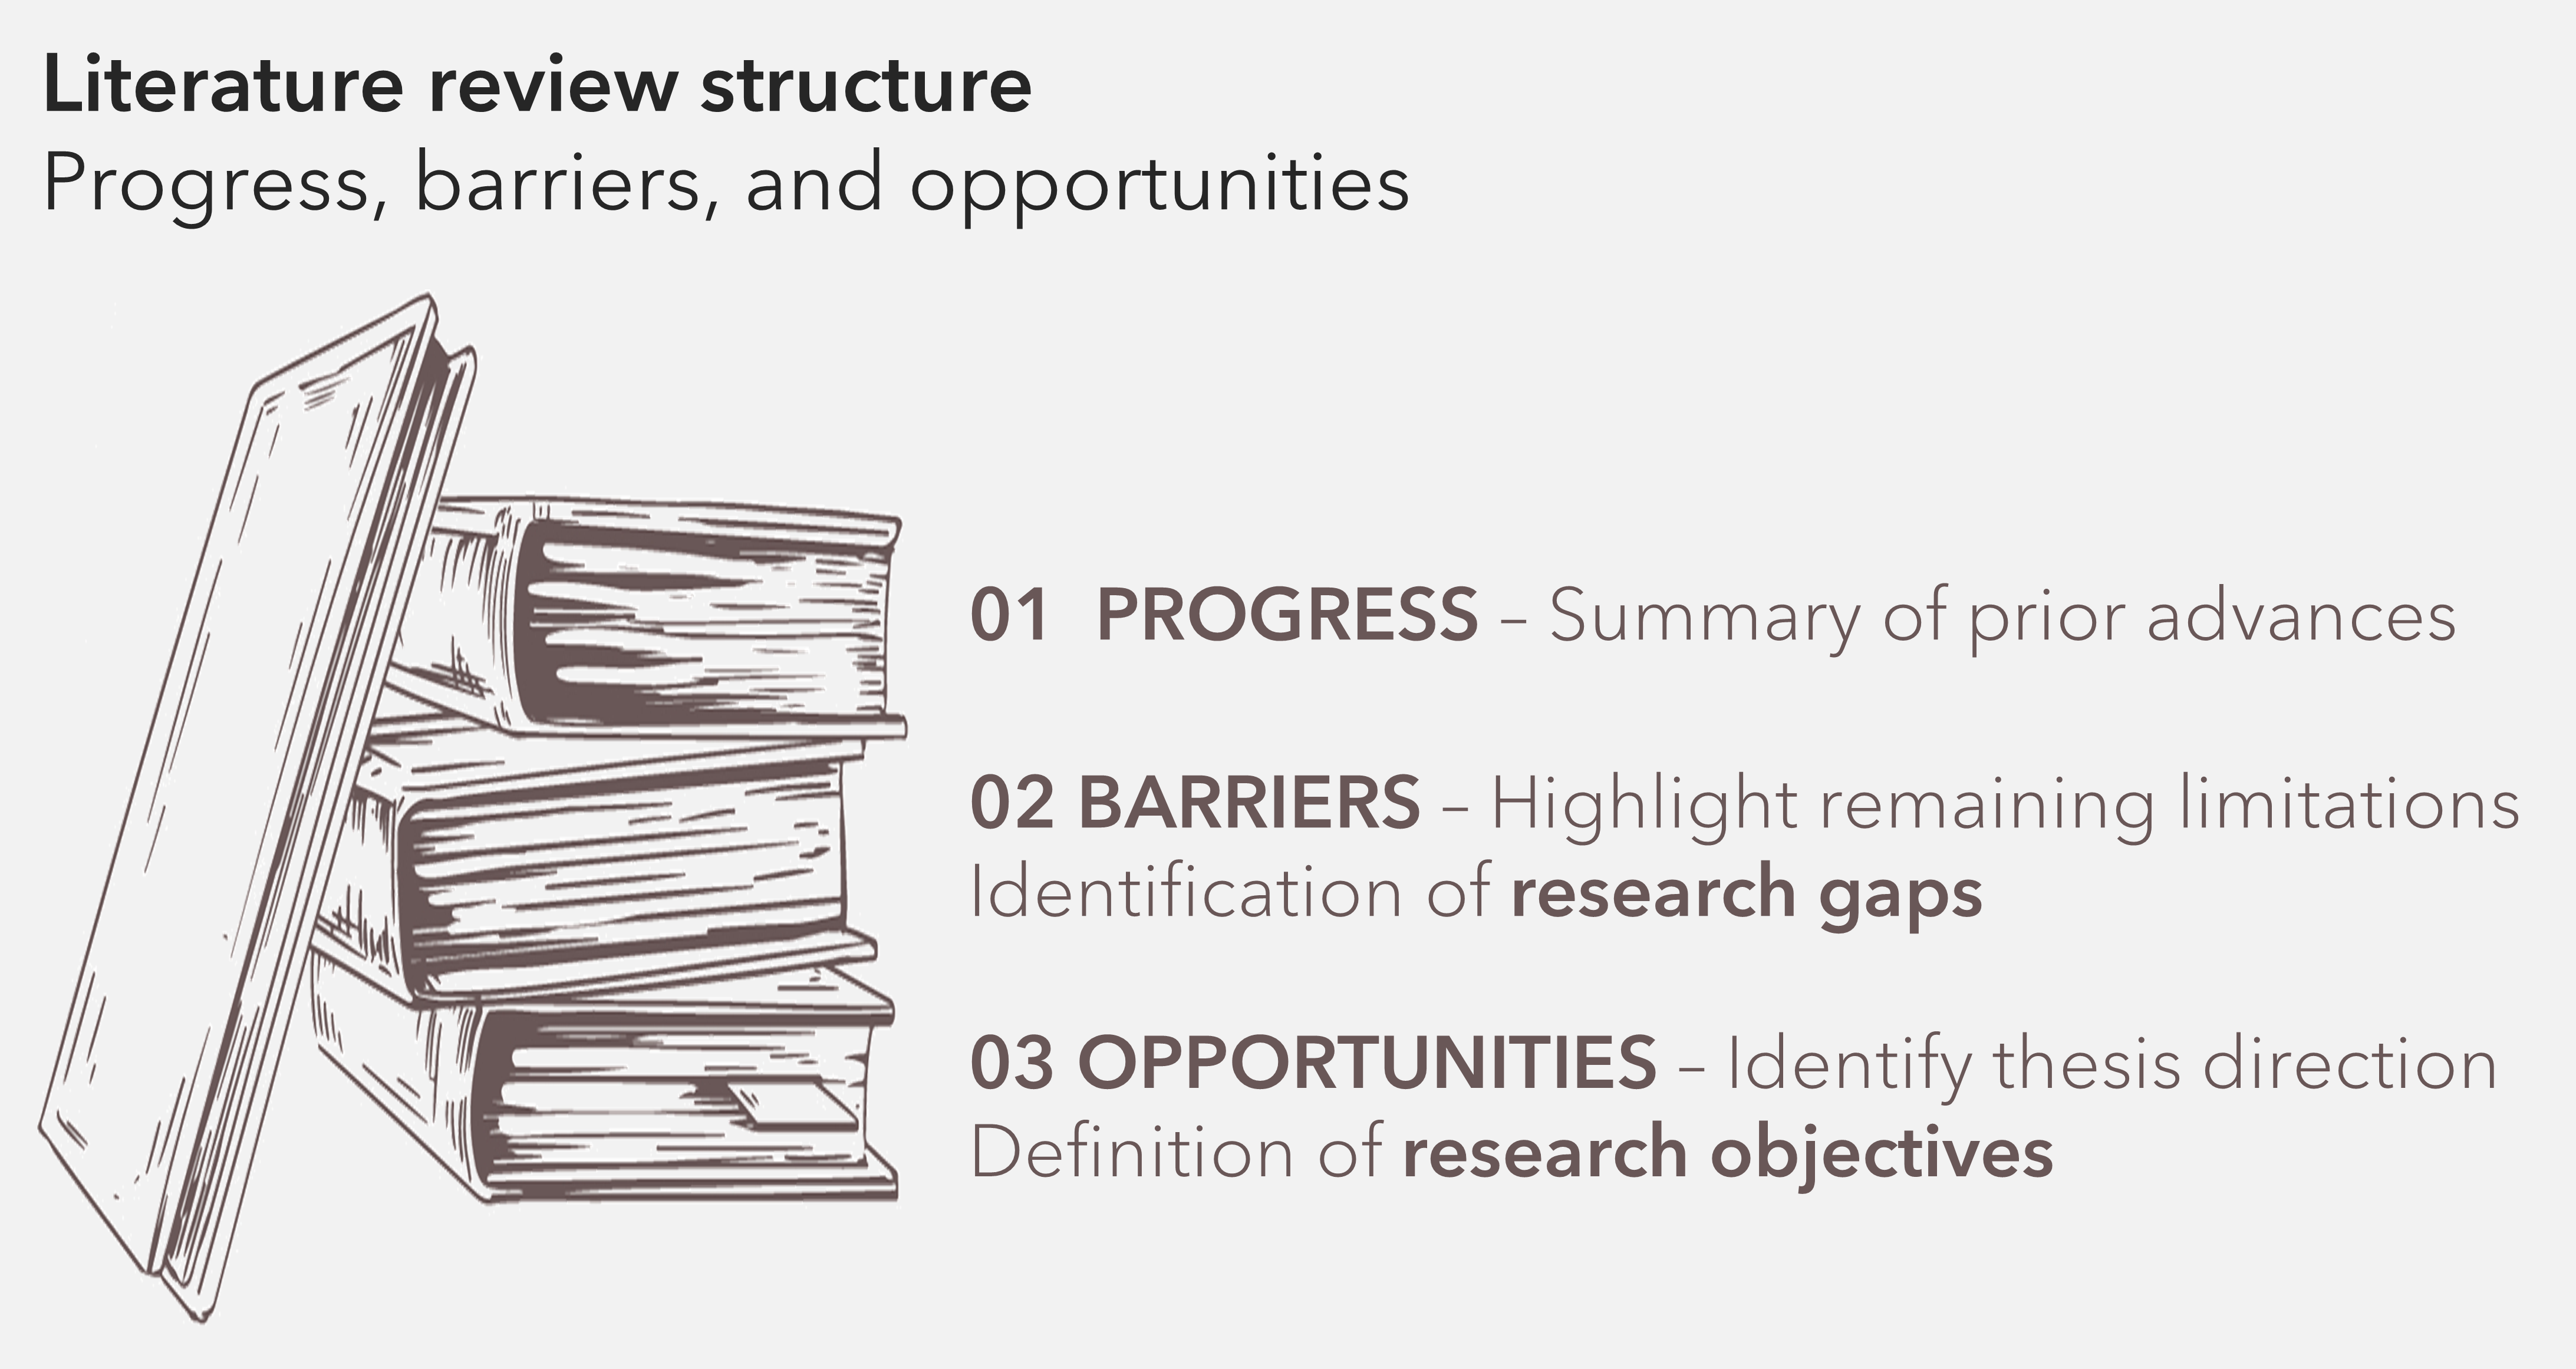
\includegraphics[scale=1.04]{Figures/Chapter_02/literature_structure.png}
\caption{\textbf{Structure of the literature review chapter}.This infographic summarises how each thematic section in the chapter is organised: “\textit{Progress}”, reviews prior work and recent advances, “\textit{Barriers}” delineates the remaining limitations and knowledge gaps, and “\textit{Opportunities}” formulates the research questions pursued in this thesis. Together, these elements guide the reader from established achievements, through current challenges, to future directions that underpin the development of a prototype flash-flood forecasting system providing medium-range forecasts over a continuous global domain.}
\label{fig:literature_structure}
\end{figure}


%%%%%%%%%%%%%%%%%%%%%%%%%%%%%%%%%%%%%%%%%%%%%%%%%%%%%%%%%%%%%%%%%%%%%%%%%%%%
\section{On the use of global NWP rainfall estimates to identify areas at risk of flash flooding}
%%%%%%%%%%%%%%%%%%%%%%%%%%%%%%%%%%%%%%%%%%%%%%%%%%%%%%%%%%%%%%%%%%%%%%%%%%%%

\subsection{Progress}

Flash floods are characterised by a rapid hydrological response to intense rainfall events, with runoff timescales ranging from mere minutes to a few hours \citep{Davis_2001}. While the interaction with local topography, land use, and drainage systems modulates flash flood severity \citep{Marchi_2010, Villacca_2025}, localised extreme rainfall has been shown to be the primary driver of flash floods\footnote{While acknowledging that flash floods can also be triggered by other mechanisms such as ice jams, dam breaks, and landslides, this thesis focuses exclusively on rainfall-triggered flash floods, as they represent the most frequent cause of these events.} \citep{Schumacher_2017, Borga_2014, Archer_2018, Meyer_2022}. Unlike riverine floods that develop gradually over many hours or days from widespread rainfall across large watersheds \citep{Wohl_2022}, flash floods generate in small catchments - typically under 100 $km^2$ or 500 $km^2$ - and within minutes to hours after the triggering rainfall event \citep{Braud_2014, Bloschl_2015}. Hence, accurately characterising and predicting localised extreme rainfall (i.e., its intensity and spatial distribution) determines our ability to identify areas at heightened risk of flash flooding . Near-perfect precision in forecasting the correct distribution of rainfall totals at the precise locations is required, as any underestimation or spatial misplacement, even by a few kilometres, can leave the interested catchment virtually dry and eliminate any flash-flood signal \citep{Nicotina_2008, Douinot_2016, Clark_2016, Wang_2022}.

Several interrelated meteorological factors contribute to extreme rainfall events’ variability in intensity and spatial distribution. The key ingredients of flash flood-producing storms are ample and persistent supply of water vapour, a mechanism to facilitate uplift of air in which the moisture condenses and precipitation forms, and a focusing mechanism (or combination of focusing mechanisms) that causes precipitation to occur continuously or repeatedly over the same area \citep{Doswell_1996}. Large-scale systems such as fronts, cyclones, and troughs can introduce substantial moisture into a region, creating conditions favourable for heavy rainfall. These systems enhance vertical motion and convective activity, leading to localised intense precipitation. Mesoscale convective systems (that is, systems with horizontal scales of 10 to 1000 km) such as squall lines and supercells can dramatically concentrate rainfall over small geographic areas, rapidly overwhelming local hydrological systems \citep{Maddox_1979, Doswell_1996, Davis_2001}. The greatest threat of excessive rainfall and significant flash flooding tends to occur when and where thunderstorms are slow-moving or stationary, continually reform over the same area, or repeatedly move over the same location. For example, if new convection develops on the storm flank opposite the direction of thunderstorm motion, then a quasi-stationary storm complex may evolve. Special circumstances exist in complex terrain where a synoptically forced flow toward and over a topographic barrier may interact with the storm dynamics. This may lead to persistent (slow-moving or quasi-stationary) and orographically enhanced storm systems that produce heavy rainfall through both increased rain rates and increased time raining over a given area Often such precipitation systems are fed by a boundary layer jet (influenced by a stalled frontal boundary) that pumps near-saturated air into the storm, thereby facilitating an efficient formation of precipitation through predominantly warm rain process at relatively low levels in the storm. Regions with an ample supply of moisture from large water bodies, whether seasonally or throughout the year, may exhibit a higher fraction of surface rainfall produced by the warm rain process (as contrasted with the “cold rain” process, which involves evolution from ice particles in the clouds). If this supply of water vapour is combined with orographic uplift (e.g., along Mediterranean coasts of Europe and Northern Africa), this may lead to very effective precipitation production and flash flooding situations.

The correct prediction of such systems remains an ongoing challenge due to the complexity of the atmospheric processes involved. To address these challenges, researchers are developing advanced forecasting tools and early warning systems that integrate high-resolution rainfall observational networks (from rain gauges or radar), km-scale NWP models, and ensemble approaches to quantify uncertainties associated with small-scale weather phenomena and provide more accurate and timely warnings for flash flood events.

For example, many studies show that to obtain better rainfall prediction of localised extreme rainfall events, in terms of location and intensity, the model's resolution must go beyond the "grey-zone" and reach values up to 1 km \citep{Castorina_2022}. These are resolutions that for global models are out of reach for at least a few more decades \citep{Wedi_2020}. Recent developments such as Destination Earth (model at 4.4 km, in the grey zone) confirms these results, as it indeed provides similar skill than the lower-resolution counter part ECMWF's IFS at 9 km. See for example the analysis for the flash floods in Valencia in 2024 \citep{Gascon}.

Flash-flood-producing convective storms have very limited predictability, and forecast skill drops sharply beyond a few hours. Due to the inherent chaotic nature of convection, small initial errors grow quickly, so accurately predicting when and where an extreme downpour will occur more than 6–12 hours in advance is extremely challenging. Indeed, inaccurate rainfall forecasting has been identified as one of the most significant sources of uncertainty in flood prediction \citep{Hapuarachchi_2011}. \citet{Schwartz_2019a, Schwartz_2019b} shows how to increase the forecasts lead times it might be necessary to reduce the members computed and reduce the spatial resolution. 

Despite the advancements produced by Km-scale NWP modelling, there remain different problems when predicting extreme rainfall. 

This motivates the shift toward probabilistic rainfall forecasts. However, even ensemble forecasts struggle with this problem. For short-range forecasts, ensemble forecasts spread can still be large, and important small-scale flash flood-triggering rainfall events may be missed in many members because the scope of the ensemble is to quantify uncertainties in rainfall prediction at its grid scale, ignoring what might be the rainfall at sub-grid scale. 

\begin{figure}[htbp]
\centering
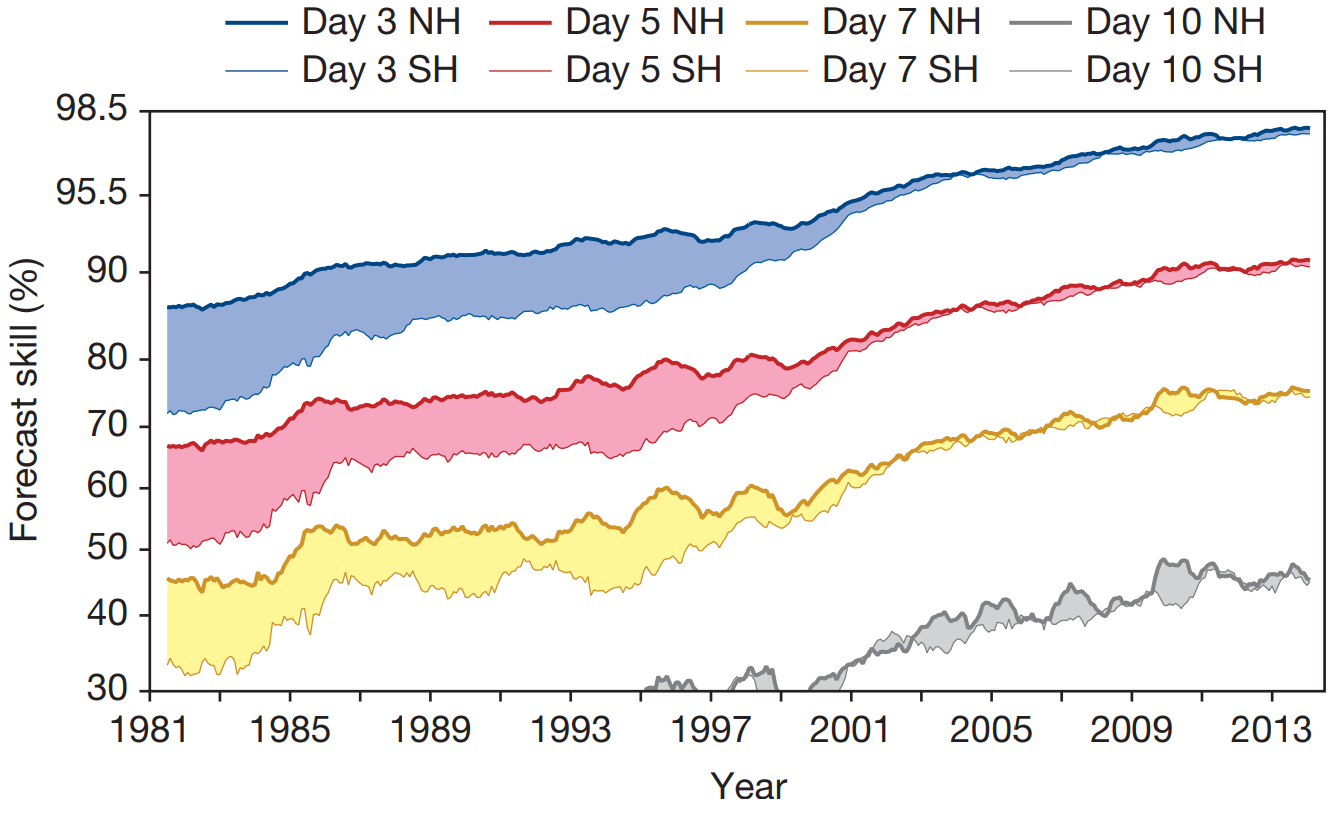
\includegraphics[width=\textwidth]{Figures/Chapter_02/improvement_forecast_skill.png}
\caption{\textbf{Forecast skill improvements for global NWP models, from \citet{Bauer_2015}}. A measure of forecast skill at three-, five-, seven- and ten-day ranges, computed over the extra-tropical northern and southern hemispheres. Forecast skill is the correlation between the forecasts and the verifying analysis of the height of the 500-hPa level, expressed as the anomaly with respect to the climatological height. Values greater than 60\% indicate useful forecasts, while those greater than 80\% represent a high degree of accuracy. The convergence of the curves for Northern Hemisphere (NH) and Southern Hemisphere (SH) after 1999 indicates the breakthrough in exploiting satellite data through the use of variational data.}
\label{fig:improvement_forecast_skill}
\end{figure}

Global NWP models could solve the issues mentioned above. They offer continuous global coverage and produce forecasts up to day 15. Their performance has been increasing steadily, one lead time every decade (Figure \ref{fig:improvement_forecast_skill}). However, for long time they have been considered not appropriate for flash flood prediction due to their coarse resolution (grid-boxes of 10+ km spatial resolution) that cannot explicitly resolve such small-scale intense convection. This often leads to missed or mislocated extreme rainfall totals in the case of small-scale convection \citep{Schumacher_2017}. This barrier is evidenced by cases of “forecast failures” for flash floods due to underestimating localised rainfall intensity, underscoring the need to overcome spatial resolution gaps. 

Notwithstanding, the interest in using rainfall estimates from NWP models has been growing due to their increased performance \citep{Bucherie_2022b}. Moreover, not necessarily coarser NWP models provide rainfall forecasts for extreme rainfall compared to higher-resolution models \citep{Hewson_2024, Wedi_2020}. Furthermore, post-processing offers a great opportunity to post-process medium-range global rainfall forecasts in order to downscale the forecasts and provide rainfall estimates for localised extreme rainfall. One notable example is the post-processing approach called ecPoint, which post-processes global model outputs to provide probabilistic rainfall forecasts at point-scale \citep{Hewson_2021}, and it has been shown to provide forecasts with better skill than raw and post-processed km-scale rainfall forecasts \citep{Gascon_2024}. 

\subsection{Barrier}
Despite the growing interest in considering rainfall estimates from global NWP models to generate forecasts over a continuous global domain and extend predictions to medium-range lead times, there is little verification of such coarser rainfall forecasts for flash flood prediction. The assessment would typically indeed be limited to rainfall observations assuming that if rainfall was correctly predicted, the model would perform equally well if used to predict flash floods \citep{Gascon_2024}. Where comparisons with areas impacted by flash floods, such comparisons are done primarily at local scale \citep{Tripathy_2020}.

While, as stated before, the main driver of flash floods is rainfall, there should be a direct assessment on the capabilities of rainfall forecasts in the prediction of flash flood events. At a local scale, many studies have assessed the capabilities of km-scale rainfall forecasts in the prediction of flash floods. The typical workflow of such studies consists in using the rainfall forecasts to verify as inputs to a hydrological model (with a more or less complex routing process) to compute discharge at a specific location. Such predicted discharge would be compared to observed discharges at the location, and scores routinely used in hydrology such as KGE or NS would be used to assess whether the magnitude of the discharge peak was correct and it was predicted with an acceptable timing. Only \citet{Herman_2018} shows rainfall verification against flash flood reports.  

There are two main problems with this workflow for the verification at a global scale of global NWP rainfall forecasts. The first one is there not exist yet a global hydrological model capable to produce discharge forecasts for small flashy catchments (i.e. below 100 km2) at global scale. Moreover, even if it was possible to create such forecasts the severe paucity of discharge observations in such small flashy catchments (which tend to be ungauged) would prevent any robust verification of such hydrological forecasts, making impossible to assess whether global NWP rainfall forecasts are suitable in identifying areas at risk of flash flooding. Even global discharge databases such as CAMELS or CARAVAN \citep{Kratzert_2023} contain less than 1\% of observations from small-flashy catchments. 

Hence, the assessment of global NWP rainfall forecasts against direct flash flood observations
remains a research gap that impedes the confident use of such forecasts to identify areas at risk of flash flooding.

\subsection{Opportunities}

The recent development of flash flood impact databases at global scale - e.g. EMDAT or Desiventar \citep{cred_2019}, continental scale - e.g., in the US or in Europe \citep{noaa_2019}, and national scale - e.g. in Ecuador  \citep{Bucherie_2022a} have opened up to the possibility of using impact flash flood data as a proxy observation for the identification of areas at risk of flash flooding. They consist in tabular data, in which each data point indicates the location (in the form of latitude/longitude coordinates) and reporting time of a reported flash flood event (including mostly the date but sometimes also the time). If the data points in such databases are pre-processed in a way that indicates in which grid-boxes flash flood events were observed (binary yes- or no-events), they could be used to run a first assessment on whether the global NWP rainfall forecasts identify the grid-boxes where the flash flood events were observed.

While it would not be possible to assess the timing, location, and magnitude of the flash flood event with score commonly used in hydrology because the rainfall is not transformed in discharge, and discharge observations are not considered, it would be possible to at least assess whether the rainfall forecasts are able to provide guidance on what are the grid-boxes likely to experience flash flooding adopting commonly used scores in probabilistic verification such as reliability diagrams, frequency bias, and roc curves. While this verification provides an outlook of flash flooding conditions, this information is useful to understand whether the rainfall forecasts contain any information regarding potential flash flooding \citep{Mason_1979}, and hence it is worth pursuing more complex hydrological modelling with such rainfall forecasts as input. 

Two aspects must be considered when implementing any verification framework using impact flash flood reports. First, this type of observations are not static like measurements coming from rain or discharge gauges, which report yes- \textit{and} no-events. With the latter is indeed possible to assess whether the model produces a correct prediction (in the case the event was or not predicted, and the event did or did not happened) or a wrong prediction (in the case the event was or not predicted, and the event did not or did happened). Impact databases include only events that \textit{were} reporter, and it is not known whether a no-report represents an event that happened but it was not reported or it represents an event that did not happen. This uncertainty makes difficult to assess whether an event was correct to not. Moreover, we do know that impact databases severely underestimate the frequency of flash flood occurrence \citep{Panwar_2020}. Hence, it is likely that any verification would overestimate the cases in which correct forecasts might be considered as wrong, undermining the assessment of the forecasts and their potential usability in the prediction of areas at risk of flash flooding. 

Despite these difficulties and including appropriate considerations around uncertainties surrounding the observational dataset, it is expected that the verification of rainfall forecast against impact flash flood reports will shed light on the capabilities of global NWP models in identifying areas at risk of flash floods. 

The research developed around this topic will be presented in chapter 5. 


%%%%%%%%%%%%%%%%%%%%%%%%%%%%%%%%%%%%%%%%%%%%%%%%%%%%%%%%%%%%%%%%%%%%%%%%%%%%
\section{On the use of reanalysis data and machine learning to create a prototype forecasting system that provides short-range predictions of areas at risk of flash flooding over a continuous global domain}
%%%%%%%%%%%%%%%%%%%%%%%%%%%%%%%%%%%%%%%%%%%%%%%%%%%%%%%%%%%%%%%%%%%%%%%%%%%%

\subsection{Progress}

In the previous section we have highlighted how important is to have rainfall forecasts that correctly locate the extreme rainfall in order to identify areas a t risk of flash flood. In this section, it will be discussed how catchment characteristics play a crucial role in determining the hydrological response to flash flood events, and how hydrologists have tried to model those interactions in order to produce flash flood predictions. 

Catchment characteristics play a crucial role in determining the hydrological response to flash flood events. The morphology, topography, land use, and soil properties of a catchment substantially influence its behaviour during extreme rainfall \citep{Henao2022, Liu2011}. Key factors such as antecedent moisture conditions, soil type, and vegetation cover are essential for evaluating runoff generation \citep{Henao2022a, Liu2011}. The scale and size of catchments add complexity to hydrological responses, with larger catchments exhibiting greater heterogeneity in their hydrodynamic behaviours \citep{Luong2021}. Catchment topography significantly modifies water movement patterns, with steeper slopes promoting quicker runoff travel times and concentrated flow pathways \citep{Liu2011, Maqtan2022a}. Soil moisture and infiltration rates are critical hydrological factors governing the occurrence and intensity of flash floods. Initial soil moisture conditions directly influence runoff generation through their effect on infiltration capacities and connectivity between surface and subsurface flow pathways \citep{Yatheendradas2008}. Flash flood forecasting systems rely heavily on accurate initial soil moisture estimates to simulate hydrological responses effectively \citep{Yatheendradas2008, AlRawas2024, Xing2019a}. Uncertainty in initial soil moisture assessments remains a challenge due to spatial heterogeneity and temporal variability in environmental factors \citep{Yatheendradas2008, AlRawas2024}. Streamflow dynamics constitute a critical aspect of hydrological factors influencing flash flood behaviour, encapsulating interactions between surface water flow and driving meteorological inputs \citep{Yang2022}. Spatial variability plays an instrumental role in shaping streamflow characteristics, with the heterogeneity of river basins affecting how water converges and accelerates in channels \citep{Zhang2024}. Accurate measurement of streamflow dynamics hinges on advancements in real-time monitoring technologies and the integration of varying data types into computationally demanding hydraulic simulations \citep{Msigwa2024, Barthold2015}.

Flash flood forecasting has evolved dramatically over the decades, transforming from basic hydrological calculations to sophisticated AI-powered prediction systems that save countless lives worldwide.

The foundations of flash flood forecasting were established through fundamental hydrological concepts developed in the mid-20th century. The unit hydrograph principle became a cornerstone concept for understanding how rainfall translates into streamflow in small watersheds \citep{Rigon2016}. These early approaches relied primarily on mathematical representations of watershed behaviour, with limited data collection capabilities and processing power. Early forecasting methods depended heavily on ground-based observations using in situ sensors, which provided relatively limited spatial coverage and temporal resolution \citep{Tao2024}. During this period, hydrologists developed theoretical frameworks that enabled more sophisticated forecasting. Concepts like lag time, storage, and the geomorphological unit hydrograph emerged as critical tools for understanding the timing and magnitude of flood responses \citep{Rigon2016}. These approaches were mostly applied to larger river systems with longer response times, leaving flash flood prediction, characterised by rapid onset and localised impacts, as a particularly challenging problem for forecasters. 

The late 20th century saw increasing efforts to translate theoretical hydrological understanding into operational forecasting systems for flash floods. This period was characterised by growing recognition of flash floods as a distinct hydrological hazard from the other types of floods, requiring specialised prediction approaches. Early warning systems during this era were primarily deterministic, using rainfall observations and simple rainfall-runoff models to predict potential flooding \citep{Hapuarachchi2011}. As computational capabilities improved in the 1980s and 1990s, more sophisticated hydrological models began to emerge, like the flash flood guidance system in the US \citep{Georgakakos_1986}. However, these early systems were limited by data availability, computational constraints, and a lack of integration between meteorological and hydrological forecasting components. Despite these limitations, they represented important steps toward developing dedicated flash flood prediction capabilities as they form the foundation of the more modern system in the 21st century. 

The beginning of the 21st century marked a pivotal moment in flash flood forecasting. A key innovation in modern flash flood forecasting systems has been their ability to integrate diverse data sources. These systems incorporate remotely-sensed precipitation data from geostationary and polar orbiter satellite platforms, reflectivity data from weather radar systems, and ground-based automated precipitation gauge measurements. This multi-source approach helped overcome the limitations of any single data type and provided more robust precipitation estimates, which are the most critical input for flood forecasting. The systems also evolved to include mesoscale NWP model forecasts integrated with land-surface model responses, enabling the creation of forecast products with longer lead times, i.e. up to 24h rather than a few hours. This integration of atmospheric and hydrologic modelling represented a significant advance over earlier, more compartmentalised approaches to flash flood prediction. The technological revolution has also played an important role in developing operational flash flood forecasting systems. As computational demands for flood forecasting increase, high-performance computing clusters become essential infrastructure for operational systems. For example, a parallel flood forecasting and warning platform, based on high-performance computing clusters, was established in China, enabling nationwide coverage with particular effectiveness for flash flood prediction. This platform utilises advanced file-based message passing on a shared hierarchical storage system, pre-allocation and dynamic allocation methods for resource management, and automatic switching between different time-scale models driven by rainfall events. These computational advances allowed for unprecedented spatial and temporal resolution in modelling, enabling more localised and accurate predictions. The ability to process vast quantities of data in near-real-time transformed the capabilities of forecasting systems, substantially reducing the gap between observation and warning issuance.

Despite the technological advances, these systems were developed for small-scale domains, such as urban, regional, or national. Urban flash flood forecasting requires specialised approaches due to complex city environments with varied land use, impermeable surfaces, and intricate drainage systems. Traditional channel models often fail to capture localised ponding scenarios independent of river overflow. Challenges include predicting pluvial flash floods, where rainfall directly generates surface runoff without channel interaction, and insufficient integration of socioeconomic vulnerability data. Innovations include high-resolution DEMs, real-time IoT sensor networks, machine learning algorithms, and ensemble precipitation modelling. Future systems must integrate hydrological observations with meteorological forecasts and regional thresholds to improve prediction accuracy in expanding urban landscapes. Regional and national forecasting systems enhanced localised flash flood prediction capabilities. These systems are designed to address their host countries or regions' specific geographic, climatic, and infrastructural conditions. By leveraging lower-resolution data inputs (e.g. from national-scale NWP models) and incorporating locally sourced datasets, they refine predictions and improve actionable outputs. The Cascading Forecasting Process, utilised within frameworks such as the Southern Africa Severe Weather Forecast Demonstration Project (SWFDP), exemplifies this approach. It facilitates the transfer of forecast outputs from advanced global centres to designated regional hubs, which interpret and provide guidance on imminent severe weather events \citep{Jubach2016}. Effective regional systems rely heavily on local ownership and accessibility of input data, often maintained under specific agreements by hydro-meteorological agencies or related institutions. This underscores the importance of robust inter-institutional collaboration \citep{Georgakakos2022}. Despite advancements in spatial resolution, adaptability, and probabilistic approaches \citep{Zanchetta2020, AlRawas2024}, challenges persist in less monitored areas where gauging stations are sparse \citep{Kuksina2020}. Addressing these observational gaps while maintaining fidelity across models tailored to specific catchments is crucial for system resilience due to climatic variability and infrastructure limitations \citep{Liu2011, Douinot2016}. 

While the theoretical and technological advances in the prediction of flash floods was important, it was still not possible to extend such complex systems at larger domains such as continental or global scale. 

From the 2010s, prototypes for continental flash flood forecasting systems started to emerged. These systems process vast amounts of global meteorological data to provide scalable predictions that can be tailored to specific regions or localised events. Operational frameworks have been established to incorporate global-to-regional interlinkages, facilitating effective information dissemination for disaster prevention initiatives at multiple scales \citep{Georgakakos2022}. However, these systems face challenges in integrating heterogeneous factors that influence flash floods, such as precipitation variability across large geographical extents and interconnected physical processes like soil permeability and lithological characteristics \citep{Henao2022, Henao2022a, Kuksina2020}. Addressing uncertainties associated with model implementations for predicting localised extreme rainfall occurrences is another fundamental consideration. Misalignments between simulated precipitation outputs and real-time weather anomalies become more pronounced at broader spatial scales \citep{Maqtan2022a, Maqtan2022b}. Continental-level systems often employ probabilistic frameworks enhanced by multi-source satellite measurement tools, such as the Integrated Multi-Satellite Retrievals for Global Precipitation Measurement (IMERG). Coupling these with emergency planning modules targeting exposure minimisation during high-risk intervals is a hallmark application that leverages global coverage advantages and computational advancements \citep{AlRawas2024}.

Such continental prototypes needed data-rich implementations. Hence, they were developed mainly in data-rich continents like the US and Europe, leaving many regions, especially in the Global South, under-covered or not protected at all. 

Physical models are a critical component of flash flood forecasting systems, employing principles derived from physical laws and equations to simulate hydrological processes. These models capture the intrinsic behaviour of natural processes such as precipitation-runoff transformations, soil infiltration, and river routing without relying on statistical or empirical relationships \citep{Hinge2024}. Operational systems like the Ensemble Framework For Flash Flood Forecasting (EF5) incorporate physical models to produce actionable runoff predictions while maintaining computational feasibility \citep{Flamig2020}, and their scalability allows for iterative improvements and parameter adjustments across diverse spatial domains \citep{Xing2019a}. Physical modelling intersects with uncertainty quantification frameworks, such as ensemble-based methods or probabilistic estimations, and systems like Flood-PROOFS utilise downscaling techniques to refine deterministic weather predictions into high-resolution forecasts for flash flood risk evaluation \citep{Zanchetta2020}. Challenges persist in achieving universality due to varying regional requirements and climatic patterns \citep{Xing2019a, AlRawas2024}. However, application frameworks like FLASH leverage ensemble configurations and physically-derived parameters to assimilate real-time meteorological inputs accurately, improving lead times for emergency alerts \citep{Martinaitis2023}. 

Data-driven models have gained prominence in flash flood forecasting due to their ability to leverage large datasets and identify complex patterns in meteorological and hydrological variables. These models employ statistical, machine learning, or neural network techniques to predict flash flood occurrences and associated risks based on historical and real-time data. A notable example is the Data-Driven Hydrological Model (DaHM), which uses a feed-forward two-layer perceptron architecture to capture non-linear relationships between input variables like precipitation and streamflow \citep{Philipp2016}. Data-driven frameworks offer the advantage of relying on empirical data rather than explicitly defined physical equations, enabling a broader range of applications where observational data is abundant \citep{Zanchetta2020, Msigwa2024}. However, their robustness is tied to the availability and quality of input datasets, and challenges arise in regions with limited historical records or sparse monitoring networks \citep{Zanchetta2020, Lu2021}. Despite inherent uncertainties in predicting localised extreme rainfall events, data-driven models continue to evolve by combining traditional observational techniques with machine learning components \citep{AlRawas2024}. Coupling data-driven models with physics-based frameworks leverages the strengths of both paradigms, fostering improvements in predictive skill and actionable knowledge dissemination \citep{Msigwa2024}. 

\subsection{Barriers}

As emerging models develop under expanding computational power and integrated datasets, there remain significant research gaps for the development of a flash flood forecasting system over a co ntinuous global domain. 

Data-driven approaches are increasingly being explored for flash flood forecasting, with the aim of overcoming limitations of traditional physics-based methods in data-sparse regions, as stated in the previous section. Recent reviews indicate that a majority of flash flood prediction studies now incorporate machine learning or artificial intelligence techniques \citep{AlRawas2024}, reflecting a shift toward data-driven modelling. Key considerations include the selection of predictive features, the scarcity and quality of historical flash flood observations, suitable forecasts, suitable model architectures, uncertainty quantification, and the computational trade-offs inherent in operationalising such a system.

A fundamental hurdle in developing data-driven flash flood models is the scarcity of reliable historical event data for model training and validation. Flash floods are relatively infrequent and highly localised, and unlike river floods, they often occur in ungauged basins with no stream gauge records of discharge or water level. Many flash flood events are documented only anecdotally (e.g., through post-event reports, disaster databases or news media) or via indirect observations (damage reports, remote sensing of flood aftermath). This leads to a paucity of labelled examples for supervised learning. The limited sample of flash flood occurrences also introduces a strong class imbalance: most time steps and locations correspond to “no flash flood” conditions, which can bias a model unless special training strategies are adopted. Some regions have assembled flash flood event catalogues — for instance, the U.S. and Europe maintain databases of flash flood reports — but globally, there is no unified flash flood archive with consistent reporting criteria. Modellers must therefore integrate heterogeneous data sources or use proxies to identify flash flood events in historical records. One feasible approach is to leverage reanalysis-driven hydrological simulations as a substitute for direct observations of flash flooding. \citet{Alkaabi2025} demonstrate this strategy in a data-sparse desert catchment: they first validated ERA5-derived runoff against a calibrated hydrologic model (HEC-HMS) for past storm events, then used the reanalysis precipitation-runoff pairs to train a deep learning model for flash flood runoff prediction. By doing so, they generated a training dataset from reanalysis that mimics the catchment’s flood response without extensive gauged flow data. Another example is the use of global runoff models or flood reanalysis products (e.g., GloFAS reanalysis) to identify periods of extreme flow that correspond to flash flooding conditions \citep{Wu2022}. While these proxies are imperfect – hydrologic models have their uncertainties – they can considerably expand the training sample size. Additionally, remote sensing offers emerging means to detect flash flood impacts (e.g., sudden increases in river turbidity or soil wetness observable by satellites), which could infer flash flood occurrences in ungauged basins for model training \citep{Smith2021}. Despite such innovations, the challenge of limited ground truth data remains a central issue for global flash flood prediction feasibility. It is difficult to capture the full spectrum of flash flood phenomena (from minor inundations to catastrophic torrents) with coarse datasets. Many events, especially in remote regions, may go unrecorded, leading to under-reporting bias. Models trained only on recorded events might struggle to predict floods in regions with no history in the dataset, even if physical conditions are ripe for flooding. Data augmentation and transfer learning become important in this context: by training on diverse climates and geographies, a model may learn general patterns that transfer to ungauged locations. Recent work in hydrology has shown that deep learning models can indeed extrapolate to ungauged basins by exploiting large training samples and catchment descriptors \citep{Kratzert2019, Gilon2024}. However, those efforts have primarily addressed riverine floods; flash floods pose additional complexity due to their rapid onset and small spatial scale. In summary, assembling a representative and extensive training dataset for global flash flood prediction is non-trivial. It likely requires combining multiple data sources (reanalysis, remote sensing, simulated events, and whatever observational records exist) to capture both positive cases (flash flood occurrences) and negatives (similar meteorological events that did not cause flooding). Careful curation of such a dataset is critical to the feasibility of any data-driven flash flood model. 

\section{Opportunities}

Applications of AI in problems with similar issues to those presented so far, i.e. severe imbalanced datasets in the prediction of lightning \citep{Cavaiola_2024} have shown the benefits of adopting machine learning algorithms to predict flash flood events. 



%%%%%%%%%%%%%%%%%%%%%%%%%%%%%%%%%%%%%%%%%%%%%%%%%%%%%%%%%%%%%%%%%%%%%%%%%%%%
\section{On the use of medium-range NWP forecasts and machine learning to assess the predictability of predictions of areas at risk of flash flooding over a continuous global domain up to medium-range lead times}
%%%%%%%%%%%%%%%%%%%%%%%%%%%%%%%%%%%%%%%%%%%%%%%%%%%%%%%%%%%%%%%%%%%%%%%%%%%%

\section{Progress}
Medium-range prediction, defined as forecasts up to 10 days ahead, has historically been elusive due to the complex, localised nature of the flash-flood-triggering rainfall events and the hydrological processes that generate the flash flood events themselves. 

Prior to the 2000s, flash flood forecasting was largely limited to very short lead times (hours to 1-2 days) due to limitations in numerical weather prediction (NWP) models and computing power. The foundations began in the 1970s with basic hydrological models and limited meteorological forecasting capabilities, exemplified by the establishment of the U.S. National Weather Service Flash Flood Program \citep{Georgakakos_1987}.

A significant shift occurred in the early 2000s, particularly after devastating floods in Europe. The development of the European Flood Alert System (EFAS) in 2003 represented one of the first major attempts at medium-range flood forecasting. This era marked the critical transition from deterministic to probabilistic forecasting approaches—a fundamental requirement for extending prediction lead times beyond 3 days. By 2020, systems like EFAS Version 4.0 introduced sub-daily calibration of hydrological models, significantly improving medium-range forecast accuracy for medium- to large-scale catchments \citep{Mazzetti_2021}. This allowed to represent medium-scale flash flood events (i.e. those where hydrological and routing processes are important), while small-scale flash floods events (i.e. primarily dependent on extreme localised rainfall events) remained largely underrepresented. At global scale, GLOFAS remain out of scope for the representation of global small- and medium-scale flash flood events. 

Several key technological breakthroughs enabled this extension from short-term to medium-range flash flood prediction: (1) ensemble prediction systems that quantify forecast uncertainty \citep{Martinaitis_2023, Flamig_2020}, (2) high-performance computing allowing more sophisticated modelling, (3) improved precipitation measurement through multi-satellite products and dual-polarization radar, (4) evolution of distributed hydrological models, and (5) the integration of machine learning and artificial intelligence techniques.


\section{Barriers}

Despite significant advances, medium-range flash flood prediction faces substantial challenges globally. While the use of medium-range global NWP models have been used since the 2000s to extend to medium-range lead time the hydrological predictions for large-scale hydrology \citep{Gouweleeuw_2005}, the primary limitation of extending hydrological predictions at all scales remains precipitation forecast uncertainty at the 5-10 day range \citep{Jasper_2002}. Hence, the cascade of uncertainty from precipitation forecasts through hydrological models continues to constrain prediction skill \citep{Georgakakos_2022a}. 

Flash floods result from convective storms that are notoriously difficult to predict beyond 1-2 days due to spatial and temporal resolution limitations of global NWP models, which typically operate at resolutions too coarse (10-25 km) to resolve the small-scale processes that trigger flash floods. However, at least at regional scale, it has been shown against flash flood impact observations that if the rainfall forecasts contain some useful guidance on the occurrence of extreme rainfall events, it is reasonable to assume that reasonable performance can be achieved at predicting areas at risk of flash floods even up to day 15 \citep{Tripathy_2020}.

Moreover, we are faced with the challenge to predict so-called "unprecedented events", events that are not present in our observational records, and people are not prepared for as shown by deadly rainfall-triggered flash floods and landslides causing hundreds of deaths and economic losses \citep{Marengo_2023, Marengo_2024, Alcantara_2023}. Future projections indeed state that we need to prepare for worse flash flood events in the near future \citep{AlRawas_2024a}.

While applied primarily for large catchments, studies show that to enhance the predictability of flood predictions, it is necessary to also quantify the uncertainty in the hydrological models to provide skillful forecasts up to day 10 \citep{Teja_2023}. However, for flash floods even the most recent developments such as EF5 \citep{Flamig_2020} provide forecasts up to 24 hours ahead, including the latest developments that use data-driven approaches \citep{Nevo_2022, Nearing_2024}. 

Hydrological model challenges include parameter uncertainty (especially for ungauged catchments), dependency on accurate initial soil moisture conditions, and scale mismatches between model resolution and the small catchments where flash floods typically occur. The combination of meteorological and hydrological uncertainties creates a cascade effect, with errors in precipitation forecasts amplifying when propagated through hydrological models. 

Regional disparities in observation networks create significant limitations for the development of a flash flood forecasting system over a continuous global domain up to medium-range lead times . While North America, Europe, and parts of East Asia benefit from dense networks of weather radars and gauges, many parts of Africa, South Asia, and South America lack adequate ground-based observation networks, particularly in mountainous areas where flash floods frequently occur. 

\section{Opportunities}

Addressing these challenges will require continued investment in high-resolution modelling, ensemble prediction systems, improved data assimilation, and machine learning techniques adapted to the specific conditions of each region, data-driven approaches could help us to make steps forward in the creation of medium-range flash flood forecasting system over a continuous global domain.

The future of medium-range flash flood prediction lies in hybrid approaches that leverage both physical understanding and data-driven insights, enhanced observational networks including non-traditional data sources, and impact-based warning frameworks that translate flood forecasts into actionable information for vulnerable communities worldwide. 

\citep{Cavaiola_2024} shows the benefits of adopting data-driven approaches in the prediction of lightning (a problem showing similar issues with imbalanced datasets) up to medium-range forecasts (although here medium-range is considered only up to t+48). 
